\documentclass[aspectratio=169]{beamer}

\usepackage{mhasbiarz}
\usepackage{booktabs}
\graphicspath{{./Images/}}

%newtheorem
\newtheorem{teorema}{Teorema}[section]
\newcommand{\lcm}{\operatorname{lcm}}
\renewcommand{\theteorema}{\arabic{section}.\arabic{teorema}}
\newtheorem{sifat}[teorema]{Sifat}
\newtheorem{akibat}[teorema]{Akibat}
\newtheorem{proposisi}[teorema]{Proposisi}
\newtheorem{definisi}[teorema]{Definisi}

%Block Baru
\newenvironment{variableblock}[3]{%
	\setbeamercolor{block body}{#2}
	\setbeamercolor{block title}{#3}
	\begin{block}{#1}}{\end{block}}

\newenvironment{rbox}[1]{
	\setbeamercolor{block body}{bg=mygreen!4,fg=black}
	\setbeamercolor{block title}{bg=mygreen!90,fg=white}
	\begin{block}{#1}}{\end{block}}

% Angka, persamaan, dan diagram di folder generated/ dibuat oleh `python -m openjackson`.
\newcommand{\PaperL}{37.49}
\newcommand{\PaperWLittle}{36.88}
\newcommand{\PaperRhoFive}{1.031}
\newcommand{\PaperPinvDiff}{2.5\times10^{-4}}
\newcommand{\RhoOne}{\frac{\lambda_{1}}{\mu_{1}}}
\newcommand{\RhoTwo}{\frac{13 \lambda_{1}}{15 \mu_{2}}}
\newcommand{\RhoThree}{\frac{2 \lambda_{1}}{3 \mu_{3}}}
\newcommand{\ExLamOne}{1.0167}
\newcommand{\ExMuOne}{1.3056}
\newcommand{\ExMuTwo}{1.2000}
\newcommand{\ExMuThree}{1.5833}
\newcommand{\ExL}{7.031}
\newcommand{\ExW}{6.92}
\newcommand{\ExWSum}{7.70}
\newcommand{\ExWSim}{6.93}
\newcommand{\ExWSimSe}{0.05}
\newcommand{\ExSimReps}{5}
\newcommand{\ExSimHorizon}{200\,000}
\newcommand{\ExSimPatients}{914\,724}
\newcommand{\CtmcCap}{50}

% Baris tabel: \@@input (primitif TeX) dapat diekspansi, jadi \midrule/\bottomrule sesudahnya tetap valid.
\makeatletter
\newcommand{\tablerows}[1]{\@@input generated/#1.tex }
\makeatother
\newcommand{\legenda}{{\footnotesize \textcolor{mygreen}{Biru putus-putus}: transisi masuk ke state; hitam: transisi keluar dari state.}}
\newcommand{\diagramstate}[1]{%
	\begin{center}
		\adjustbox{max width=\linewidth, max totalheight=0.72\textheight}{\input{generated/diagram-#1}}
	\end{center}
	\legenda}

\begin{document}
\title{\color{mygreen} Riset Operasi B}
\subtitle{\color{mygreen!90} Kelompok 4}

\author[mhasbiarz]{\color{black}
Ridho Maulana Asrofi \\
Aprila Adzkiyan Najah \\
Nala Kirana Prastiwi \\
Delia Noor Mavianti \\
Moh Hasbi Alfarizi }

\date{{\footnotesize \color{mygreen!90}} }

\subject{}
\titlegraphic{\begin{tikzpicture}[overlay, remember picture]
		\node[xshift=5cm,yshift=-8.02cm]{
\includegraphics[width=12cm]{img1}
		};
	\end{tikzpicture}
	\begin{tikzpicture}[overlay, remember picture]
		\node[xshift=11cm,yshift=-4mm]{
\includegraphics[width=5cm]{logo}
		};
	\end{tikzpicture}
}

\maketitle

\begin{frame}
    \begin{center}
    \color{mygreen} \huge \textbf{On the Application of the Open Jackson Queuing Network in Hospital}
    \end{center}
    \begin{center}
        Arum Helmi Manggala Putri, Irwan Endrayanto
    \end{center}
    \begin{center}
        \color{mygreen!90} \large Kelompok 4
    \end{center}
\end{frame}

\begin{frame}{Table of Contents}
	\begin{multicols}{2}
		\tableofcontents
	\end{multicols}
\end{frame}

\section{\color{mygreen}\huge Pendahuluan}
\begin{frame}{Pendahuluan}
Open Jackson queuing network adalah sistem antrian baris terbuka yang terdiri dari beberapa stasiun layanan. Pada open Jackson queuing network, pasien tiba dari luar sistem untuk mendapatkan layanan dan kemudian meninggalkan sistem. Teori open Jackson queuing network digunakan untuk menentukan model sistem antrian yang akan dibangun berdasarkan diagram tahap layanan di rumah sakit.
\end{frame}


\section{\color{mygreen}\huge Rumusan Masalah}
\begin{frame}{Rumusan Masalah}
\begin{itemize}
    \item Apakah yang dimaksud dengan open Jackson queuing network?
    \item Bagaimana model open Jackson queuing network dapat diterapkan untuk menentukan model sistem antrian layanan di rumah sakit, dan bagaimana balance equations-nya?
    \item Apakah hasil numerik paper (probabilitas perpindahan antarstasiun, jumlah rata-rata pasien, dan waktu tunggu) dapat direproduksi?
\end{itemize}
\end{frame}


\section{\color{mygreen}\huge Studi Literatur}
\begin{frame}{Studi Literatur}
\begin{rbox}{Model Jaringan Antrian di Rumah Sakit}
\justifying Fenomena antrian dapat terjadi ketika permintaan suatu layanan melebihi kapasitas yang tersedia. Antrian pasien di rumah sakit untuk mendapatkan layanan medis menyebabkan pasien kehilangan waktu, tenaga, biaya, dan menurunnya tingkat kepercayaan pasien terhadap rumah sakit. Oleh karena itu, diperlukan teori antrian untuk memberikan gambaran atau model terkait permasalahan sistem antrian.

Penelitian ini mengadopsi Open Jackson Queueing Network untuk memodelkan dan menganalisis sistem antrian yang ada dengan tujuan pasien mendapatkan rasa nyaman dan puas terhadap pelayanan yang diberikan.
\end{rbox}
\end{frame}

\begin{frame}{Studi Literatur}
\begin{rbox}{Open Jackson Queueing Network}
\justifying Open Jackson Queueing Network adalah jaringan yang terdiri dari $N$ stasiun dengan satu server. Kedatangan dari luar jaringan ke stasiun $i$, $i = 1,2,\dots,N$, mengikuti proses Poisson dengan laju $\lambda_{0i}$ ($\lambda_{0i} \geq 0$). Waktu layanan di stasiun $i$ berdistribusi eksponensial dengan laju $\mu_i$ (rata-rata waktu layanan $1/\mu_i$).

Setelah dilayani di stasiun $i$, pasien berpindah ke stasiun $j$ dengan probabilitas $p_{ij}$ $(0 \leq p_{ij} \leq 1)$, saling bebas. Parameter $p_{i0} = 1 - \sum_{j} p_{ij}$ menyatakan proporsi pasien yang meninggalkan jaringan setelah dilayani di stasiun $i$. Laju kedatangan total $\lambda_j$ di stasiun $j$ memenuhi \emph{traffic equations}
\[
    \lambda_j = \lambda_{0j} + \sum_{i=1}^{N} \lambda_i p_{ij}, \qquad j = 1,2,\dots,N.
\]
\end{rbox}
\end{frame}

\begin{frame}{Studi Literatur}
\begin{rbox}{Teorema Jackson}
    \justifying Laju $\lambda_j$ terdiri dari kedatangan ke stasiun $j$ dari luar dan dari dalam jaringan. Jaringan antrian dengan karakteristik ini disebut Open Jackson Queueing Network. Menurut teorema Jackson, jika $\rho_i = \lambda_i/\mu_i < 1$ untuk setiap $i$, distribusi stasioner jaringan dengan $N$ stasiun satu server berbentuk produk
    \[
        P(n_1,\dots,n_N) = \prod_{i=1}^N (1-\rho_i)\,\rho_i^{n_i}, \qquad n_i \geq 0,
    \]
    dengan $P(n_1,\dots,n_N)$ peluang terdapat $n_i$ pasien di stasiun $i$ untuk setiap $i = 1,2,\dots,N$. Jadi setiap stasiun berperilaku seperti antrean M/M/1 yang saling bebas.
\end{rbox}
\end{frame}

\begin{frame}{Studi Literatur}
\begin{rbox}{Analisis Antrian Satu Server M/M/1 : (FCFS/$\infty$/$\infty$)}
    Karakteristik dan asumsi dari model antrian di semua stasiun layanan dapat disimpulkan menjadi notasi Kendall $(M/M/1)$: (FCFS/$\infty$/$\infty$): kedatangan mengikuti proses Poisson (waktu antar-kedatangan berdistribusi eksponensial) dan waktu layanan berdistribusi eksponensial. Selain itu, setiap stasiun layanan hanya memiliki satu server, dan kapasitas antrean serta sumber pasien tidak terbatas.
    \begin{figure}
        \centering
        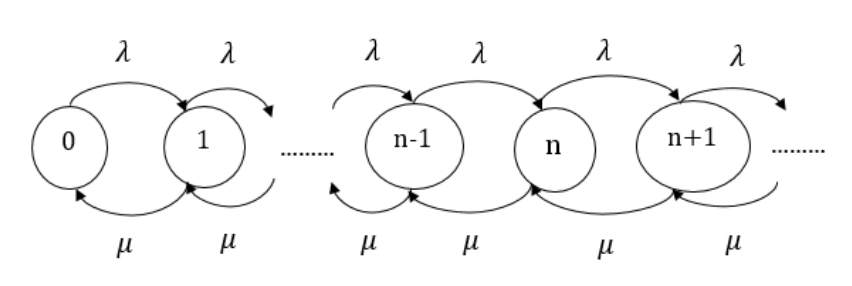
\includegraphics[width=0.38\linewidth]{mm1.PNG}
        \caption{Diagram Transisi State di Antrean M/M/1}
    \end{figure}
\end{rbox}
\end{frame}

\begin{frame}{{Studi Literatur}}
\begin{rbox}{Analisis Antrian Satu Server M/M/1 : (FCFS/$\infty$/$\infty$)}
    Berdasarkan Gambar 1, sistem berada dalam keseimbangan statistik ketika laju aliran dari state $n-1$ ke $n$ sama dengan laju aliran dari $n$ ke $n-1$ untuk setiap $n = 1,2,3,\dots$. Keseimbangan statistik ini menghasilkan balance equation lokal
    \[
        \lambda P_{n-1} = \mu P_n,\quad n \geq 1
        \qquad\Longrightarrow\qquad
        P_n = \rho^n P_0 = (1-\rho)\,\rho^n,\quad \rho = \frac{\lambda}{\mu} < 1.
    \]
    Akibatnya jumlah rata-rata pasien $L = \sum_n n P_n = \dfrac{\rho}{1-\rho}$ dan, dengan hukum Little, waktu rata-rata di sistem $W = \dfrac{L}{\lambda} = \dfrac{1}{\mu-\lambda}$.
\end{rbox}
\end{frame}

\section{\color{mygreen}\huge Pembahasan}
\begin{frame}{Pembahasan}
    \begin{rbox}{Diagram Skematik Jaringan Antrean di Fasilitas Rumah Sakit}
        Jaringan antrean di rumah sakit ini terdiri dari beberapa ruangan layanan, di antaranya adalah \textcolor{red}{ruang registrasi}, \textcolor{red}{ruang pemeriksaan (oleh perawat)}, \textcolor{red}{ruang pemeriksaan (oleh dokter)}, dan \textcolor{red}{ruang administrasi serta farmasi}. Tingkat kedatangan pelanggan di setiap ruang layanan ditandai dengan $\lambda_i$ dan tingkat keberangkatan pelanggan ditandai dengan $\mu_i$ dengan $i = 1,2,3, \dots$ Diagram skema jaringan di rumah sakit diberikan pada gambar sebagai berikut:
    \end{rbox}
\end{frame}

\begin{frame}{Pembahasan}
        \centering
        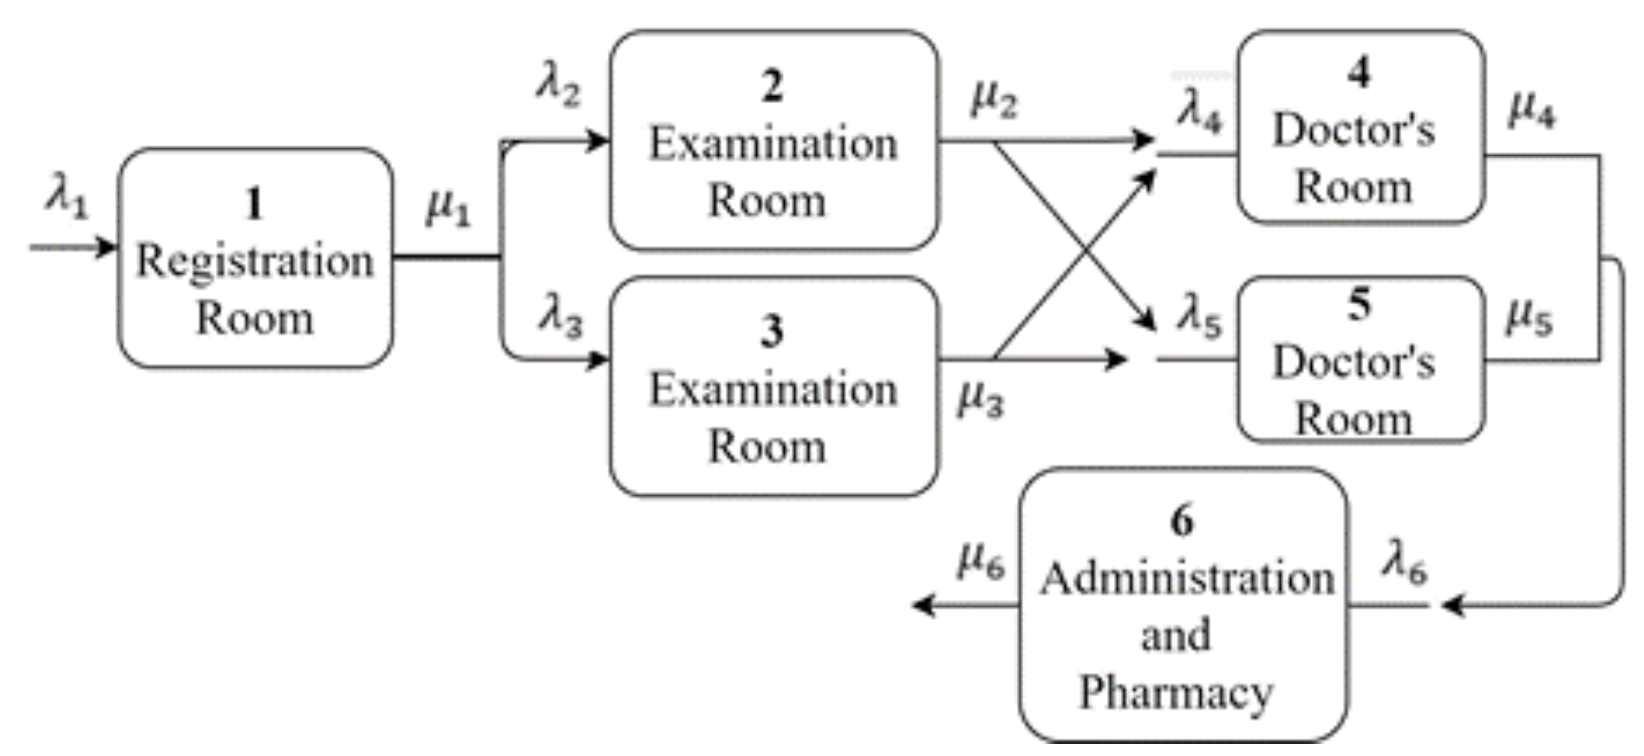
\includegraphics[width=0.5\linewidth]{Diagram Skematik.png}

        {\footnotesize Sumber: Putri dan Endrayanto.}

    \justifying Namun, untuk kasus jaringan seperti diagram di atas perhitungannya terlalu kompleks, sehingga hanya diambil beberapa bagian saja agar perhitungannya lebih sederhana, yang diberikan pada Gambar 2 berikut.

\end{frame}

\begin{frame}{Diagram}
Pasien yang datang harus melewati service unit 1, yaitu ruang registrasi. Selanjutnya $\tfrac13$ pasien menuju service unit 2 (ruang dokter) dan $\tfrac23$ menuju service unit 3 (ruang laboratorium). Dari unit 3, $\tfrac45$ pasien menuju unit 2 karena masih memerlukan dokter dan $\tfrac15$ keluar. Pasien keluar dari sistem setelah dilayani di unit 2.
   \begin{figure}
        \centering
        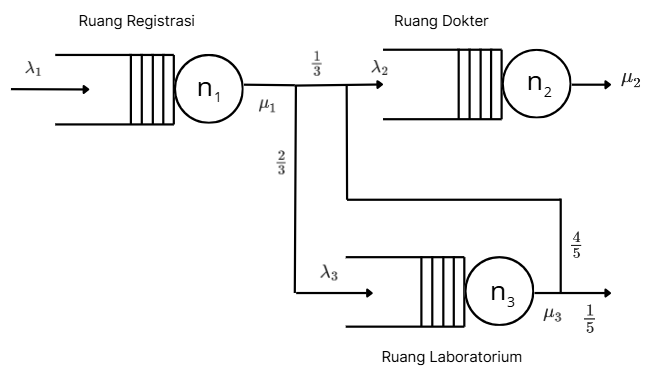
\includegraphics[width=0.42\linewidth]{diagram 1.PNG}
        \caption{Diagram Skematik Jaringan Antrian Sederhana di Rumah sakit}
    \end{figure}
\end{frame}

\begin{frame}{Pembahasan}
    \begin{rbox}{Jenis Model dan Asumsi}
    Jenis model antrean yang digunakan pada penelitian ini adalah model antrean \textbf{M/M/1}: setiap \textit{server station} terdiri dari satu \textit{server}, kedatangan pasien dari luar mengikuti proses Poisson dengan laju $\lambda_1$, dan waktu layanan di stasiun $i$ berdistribusi eksponensial dengan laju $\mu_i$.\\[1ex]
    Adapun asumsi-asumsi yang digunakan pada penelitian ini yaitu:
    \begin{enumerate}
        \item [(1)] \textbf{\textit{No reneging}} atau pasien tidak meninggalkan antrian walaupun telah menunggu lama untuk mendapatkan layanan.
        \item [(2)] \textbf{\textit{No balking}} atau pasien yang datang selalu masuk antrian, sepanjang apa pun antriannya.
    \end{enumerate}
    \end{rbox}
\end{frame}

\begin{frame}{STATE SPACE}
  Notasi $n_{i}(t)$ menyatakan banyaknya pasien di service unit $i$ pada waktu $t$, baik yang sedang menunggu maupun yang sedang dilayani:
  \begin{enumerate}
      \item $n_{1}(t)$: service unit 1 (ruang registrasi).
      \item $n_{2}(t)$: service unit 2 (ruang dokter).
      \item $n_{3}(t)$: service unit 3 (ruang laboratorium).
  \end{enumerate}
  State space-nya adalah $S = \{(n_1,n_2,n_3) : n_1,n_2,n_3 \in \{0,1,2,\dots\}\}$.
\end{frame}

\begin{frame}{TRANSITION STATE}
Berikut merupakan transition state dari diagram antrian di rumah sakit:
\begin{table}[h]
\centering
\begin{tabular}{cccc}
\toprule
\textbf{Dari} & \textbf{Menuju} & \textbf{Rate} & \textbf{Syarat} \\
\midrule
\tablerows{transitions}
\bottomrule
\end{tabular}
\caption{Tabel transition state}
\end{table}
\end{frame}

\section{\color{mygreen}\huge Diagram Transition}
\begin{frame}{Diagram Transition: $(n_1,n_2,n_3)$}
    \diagramstate{5}
\end{frame}

\begin{frame}{Diagram Transition: $(0,0,0)$}
    \diagramstate{1}
\end{frame}

\begin{frame}{Diagram Transition: $(n_1,0,0)$}
    \diagramstate{2}
\end{frame}

\begin{frame}{Diagram Transition: $(0,n_2,0)$}
    \diagramstate{3}
\end{frame}

\begin{frame}{Diagram Transition: $(0,0,n_3)$}
    \diagramstate{4}
\end{frame}

\begin{frame}{Diagram Transition: $(n_1,n_2,0)$}
    \diagramstate{6}
\end{frame}

\begin{frame}{Diagram Transition: $(0,n_2,n_3)$}
    \diagramstate{7}
\end{frame}

\begin{frame}{Diagram Transition: $(n_1,0,n_3)$}
    \diagramstate{8}
\end{frame}


\section{\color{mygreen}\huge Balance equations}
\begin{frame}{Balance Equations}
    Laju keluar dari suatu state sama dengan laju masuk ke state tersebut:
    \small
    \begin{enumerate}
        \item Kasus $n_{1}=0,\ n_{2}=0,\ n_{3}=0$ \[
\begin{aligned}
  \lambda_{1}\,P_{0,0,0} &= \mu_{2}\,P_{0,1,0} + \tfrac{1}{5}\mu_{3}\,P_{0,0,1}
\end{aligned}
\]

        \item Kasus $n_{1}>0,\ n_{2}=0,\ n_{3}=0$ \[
\begin{aligned}
  (\lambda_{1} + \mu_{1})\,P_{n_{1},0,0} &= \lambda_{1}\,P_{n_{1}-1,0,0} + \mu_{2}\,P_{n_{1},1,0} + \tfrac{1}{5}\mu_{3}\,P_{n_{1},0,1}
\end{aligned}
\]

        \item Kasus $n_{1}=0,\ n_{2}>0,\ n_{3}=0$ \[
\begin{aligned}
  (\lambda_{1} + \mu_{2})\,P_{0,n_{2},0} &= \tfrac{1}{3}\mu_{1}\,P_{1,n_{2}-1,0} + \mu_{2}\,P_{0,n_{2}+1,0} + \tfrac{1}{5}\mu_{3}\,P_{0,n_{2},1}\\
  &\quad + \tfrac{4}{5}\mu_{3}\,P_{0,n_{2}-1,1}
\end{aligned}
\]

    \end{enumerate}
\end{frame}

\begin{frame}{Balance Equations}
    \small
    \begin{enumerate}
        \setcounter{enumi}{3}
        \item Kasus $n_{1}=0,\ n_{2}=0,\ n_{3}>0$ \[
\begin{aligned}
  (\lambda_{1} + \mu_{3})\,P_{0,0,n_{3}} &= \tfrac{2}{3}\mu_{1}\,P_{1,0,n_{3}-1} + \mu_{2}\,P_{0,1,n_{3}} + \tfrac{1}{5}\mu_{3}\,P_{0,0,n_{3}+1}
\end{aligned}
\]

        \item Kasus $n_{1}>0,\ n_{2}>0,\ n_{3}>0$ \[
\begin{aligned}
  (\lambda_{1} + \mu_{1} + \mu_{2} + \mu_{3})\,P_{n_{1},n_{2},n_{3}} &= \lambda_{1}\,P_{n_{1}-1,n_{2},n_{3}} + \tfrac{1}{3}\mu_{1}\,P_{n_{1}+1,n_{2}-1,n_{3}} + \tfrac{2}{3}\mu_{1}\,P_{n_{1}+1,n_{2},n_{3}-1}\\
  &\quad + \mu_{2}\,P_{n_{1},n_{2}+1,n_{3}} + \tfrac{1}{5}\mu_{3}\,P_{n_{1},n_{2},n_{3}+1} + \tfrac{4}{5}\mu_{3}\,P_{n_{1},n_{2}-1,n_{3}+1}
\end{aligned}
\]

        \item Kasus $n_{1}>0,\ n_{2}>0,\ n_{3}=0$ \[
\begin{aligned}
  (\lambda_{1} + \mu_{1} + \mu_{2})\,P_{n_{1},n_{2},0} &= \lambda_{1}\,P_{n_{1}-1,n_{2},0} + \tfrac{1}{3}\mu_{1}\,P_{n_{1}+1,n_{2}-1,0} + \mu_{2}\,P_{n_{1},n_{2}+1,0}\\
  &\quad + \tfrac{1}{5}\mu_{3}\,P_{n_{1},n_{2},1} + \tfrac{4}{5}\mu_{3}\,P_{n_{1},n_{2}-1,1}
\end{aligned}
\]

    \end{enumerate}
\end{frame}

\begin{frame}{Balance Equations}
    \small
    \begin{enumerate}
        \setcounter{enumi}{6}
        \item Kasus $n_{1}=0,\ n_{2}>0,\ n_{3}>0$ \[
\begin{aligned}
  (\lambda_{1} + \mu_{2} + \mu_{3})\,P_{0,n_{2},n_{3}} &= \tfrac{1}{3}\mu_{1}\,P_{1,n_{2}-1,n_{3}} + \tfrac{2}{3}\mu_{1}\,P_{1,n_{2},n_{3}-1} + \mu_{2}\,P_{0,n_{2}+1,n_{3}}\\
  &\quad + \tfrac{1}{5}\mu_{3}\,P_{0,n_{2},n_{3}+1} + \tfrac{4}{5}\mu_{3}\,P_{0,n_{2}-1,n_{3}+1}
\end{aligned}
\]

        \item Kasus $n_{1}>0,\ n_{2}=0,\ n_{3}>0$ \[
\begin{aligned}
  (\lambda_{1} + \mu_{1} + \mu_{3})\,P_{n_{1},0,n_{3}} &= \lambda_{1}\,P_{n_{1}-1,0,n_{3}} + \tfrac{2}{3}\mu_{1}\,P_{n_{1}+1,0,n_{3}-1} + \mu_{2}\,P_{n_{1},1,n_{3}}\\
  &\quad + \tfrac{1}{5}\mu_{3}\,P_{n_{1},0,n_{3}+1}
\end{aligned}
\]

    \end{enumerate}
\end{frame}


\section{\color{mygreen}\huge Bentuk Produk}
\begin{frame}{Solusi Bentuk Produk}
\begin{rbox}{Traffic equations}
    Dengan $p_{12} = \tfrac13$, $p_{13} = \tfrac23$, $p_{32} = \tfrac45$ dan kedatangan dari luar hanya ke unit 1:
    \[
        \lambda_3 = \tfrac23\lambda_1, \qquad \lambda_2 = \tfrac13\lambda_1 + \tfrac45\lambda_3 = \tfrac{13}{15}\lambda_1,
        \qquad \rho_1 = \RhoOne,\quad \rho_2 = \RhoTwo,\quad \rho_3 = \RhoThree.
    \]
\end{rbox}
\begin{rbox}{Teorema Jackson}
    Jika $\rho_1,\rho_2,\rho_3 < 1$, maka
    $P_{n_1,n_2,n_3} = (1-\rho_1)\rho_1^{n_1}\,(1-\rho_2)\rho_2^{n_2}\,(1-\rho_3)\rho_3^{n_3}$.
    Substitusi ke kedelapan balance equations menghasilkan identitas (dicek secara simbolik).
    Jumlah rata-rata pasien $L = \sum_i \frac{\rho_i}{1-\rho_i}$ dan waktu rata-rata di sistem $W = L/\lambda_1$ (hukum Little).
\end{rbox}
\end{frame}

\begin{frame}{Contoh Numerik}
    Laju ilustrasi (pasien/menit): $\lambda_1 = \ExLamOne$, $\mu_1 = \ExMuOne$ (stasiun 1 paper), $\mu_2 = \ExMuTwo$ (gabungan dua ruang dokter), $\mu_3 = \ExMuThree$ (gabungan dua ruang pemeriksaan).
    \begin{table}
        \small
        \begin{tabular}{lccccc}
            \toprule
            Stasiun & $\lambda_i$ & $\rho_i$ & \makecell{$L_i$\\bentuk produk} & \makecell{$L_i$ CTMC\\($n_i \le \CtmcCap$)} & \makecell{$L_i$\\simulasi} \\
            \midrule
            \tablerows{example}
            \bottomrule
        \end{tabular}
    \end{table}
    \footnotesize
    $W = L/\lambda_1 = \ExW$ menit; simulasi \ExSimReps{} kali $\times$ \ExSimHorizon{} menit (\ExSimPatients{} pasien) memberi $\ExWSim \pm \ExWSimSe$ menit. Menjumlahkan $1/(\mu_i-\lambda_i)$ ketiga stasiun memberi \ExWSum{} menit, terlalu besar karena tidak setiap pasien melewati setiap stasiun.
\end{frame}

\begin{frame}{Verifikasi Numerik}
    Rantai Markov dipotong pada paling banyak $c$ pasien per stasiun, lalu $\pi Q = 0$ diselesaikan tanpa memakai bentuk produk. Hasilnya mendekati bentuk produk ketika $c$ membesar.
    \begin{table}
        \small
        \begin{tabular}{rrccccc}
            \toprule
            $c$ & State & $L_1$ & $L_2$ & $L_3$ & $L$ & Galat relatif maks. $P_{n}$, $n_i \le 5$ \\
            \midrule
            \tablerows{ctmc}
            \midrule
            $\infty$ & & \multicolumn{4}{c}{bentuk produk: $L = \ExL$} & \\
            \bottomrule
        \end{tabular}
    \end{table}
\end{frame}


\section{\color{mygreen}\huge Reproduksi Paper}
\begin{frame}{Reproduksi Paper: Laju Kedatangan dan Layanan}
    Semua nilai tabel paper didapat kembali dengan $\lambda_i = \text{kedatangan}/180$ dan $\mu_i = \text{keberangkatan}/180$ (observasi 3 jam, pasien/menit).
    \begin{table}
        \small
        \begin{tabular}{ccccccc}
            \toprule
            Stasiun & Kedatangan & Keberangkatan & $\lambda_i$ & $\mu_i$ & $\rho_i$ paper & $\rho_i = \lambda_i/\mu_i$ \\
            \midrule
            \tablerows{paper-rates}
            \bottomrule
        \end{tabular}
    \end{table}
    \footnotesize Nilai $\rho_i$ pada paper dipotong (bukan dibulatkan) ke 4 desimal, misalnya $0.4722/0.7722 = 0.61150$ ditulis $0.6114$.
\end{frame}

\begin{frame}{Reproduksi Paper: Probabilitas Perpindahan}
    \small
    Paper menyusun 11 persamaan untuk 9 probabilitas, $\lambda_j = \sum_i \mu_i P_{ij}$ ($j = 2,\dots,6$) dan $\mu_i = \sum_j \mu_i P_{ij}$ ($i = 1,\dots,6$), lalu menyelesaikannya dengan pseudo-invers Moore--Penrose ($P = A^{+} b$).
    \begin{columns}[T]
        \begin{column}{0.5\linewidth}
            \centering\footnotesize
            \begin{tabular}{cccc}
                \toprule
                & $A^{+}b$ & Dinormalisasi & Paper \\
                \midrule
                \tablerows{paper-routing}
                \bottomrule
            \end{tabular}
        \end{column}
        \begin{column}{0.46\linewidth}
            \footnotesize
            \begin{itemize}
                \item $A^{+}$ paper tereproduksi (selisih maks.\ $\PaperPinvDiff$).
                \item Angka paper adalah $A^{+}b$ yang dua cabangnya di stasiun 1, 2, dan 3 dinormalisasi agar berjumlah 1. Langkah ini tidak disebutkan.
                \item Pangkat $A$ hanya 8, jadi $P_{24}, P_{25}, P_{34}, P_{35}$ tidak tunggal; pseudo-invers memilih norma terkecil.
                \item Slide awal menulis $\mu_3 P_{35}$ di baris $\lambda_6$; $A^{+}$ paper dihitung tanpa suku itu.
            \end{itemize}
        \end{column}
    \end{columns}
\end{frame}

\begin{frame}{Reproduksi Paper: Jumlah Pasien dan Waktu Tunggu}
    \begin{table}
        \footnotesize
        \begin{tabular}{ccccc|cc}
            \toprule
            & \multicolumn{4}{c|}{Dengan $\lambda_i$ terukur} & \multicolumn{2}{c}{Traffic equations, $P_{ij}$ paper} \\
            Stasiun & $\lambda_i$ & $L_i$ & $L_i$ dibulatkan & $W_i = L_i/\lambda_i$ & $\lambda_i$ & $\rho_i$ \\
            \midrule
            \tablerows{paper-stations}
            \bottomrule
        \end{tabular}
    \end{table}
    \footnotesize
    \begin{itemize}
        \item $L = 39$ pada paper adalah jumlah $L_i$ yang dibulatkan; tanpa pembulatan $L = \PaperL$.
        \item $W = 54.61$ menit pada paper adalah jumlah $W_i$ keenam stasiun, seolah setiap pasien melewati semua stasiun. Setiap pasien hanya melewati 4 stasiun; dengan hukum Little $W = L/\lambda_1 = \PaperWLittle$ menit.
        \item Dengan $P_{ij}$ paper, traffic equations memberi $\rho_5 = \PaperRhoFive > 1$: stasiun 5 tidak stabil.
    \end{itemize}
\end{frame}


\section{\color{mygreen}\huge Kesimpulan}
\begin{frame}{Kesimpulan}
    \begin{itemize}
        \item Jaringan registrasi--dokter--laboratorium adalah open Jackson network tiga stasiun M/M/1 dengan $\lambda_2 = \tfrac{13}{15}\lambda_1$ dan $\lambda_3 = \tfrac23\lambda_1$. Jaringan stabil jika $\lambda_1 < \mu_1$, $13\lambda_1 < 15\mu_2$, dan $2\lambda_1 < 3\mu_3$.
        \item Balance equations untuk kedelapan kasus state dipenuhi oleh solusi bentuk produk Jackson, dan hasil ini dicek secara simbolik, dengan rantai Markov terpotong, dan dengan simulasi.
        \item Tabel laju, pseudo-invers, dan probabilitas perpindahan paper dapat direproduksi. Namun jumlah rata-rata pasien adalah \PaperL{} (paper: 39, hasil pembulatan), waktu rata-rata di sistem \PaperWLittle{} menit (paper: 54.61), dan probabilitas perpindahan paper membuat stasiun 5 tidak stabil.
    \end{itemize}
\end{frame}

\begin{frame}
	
	\begin{tikzpicture}[overlay, remember picture]
		\node[xshift=5cm,yshift=-5.32cm]{
\includegraphics[width=12cm]{img1}
		};
	\end{tikzpicture}

	\begin{tikzpicture}[overlay, remember picture]
		\node[xshift=4.1cm,yshift=0mm]{
\includegraphics[width=7cm]{Ty}
		};
	\end{tikzpicture}

	\hspace{8 cm}\textit{\color{mygreen}\huge Terima {\color{mygreen!50}Kasih}}
\end{frame}

\end{document}
